\documentclass[10pt,a4paper]{article}
\usepackage[top=3cm,bottom=3cm,includeheadfoot]{geometry}	% Seitengeometrie festlegen
\usepackage[ngerman]{babel}
\usepackage{fancyhdr}						% das nötige Paket um Fuß- / Kopfzeilen zu verwenden			
\usepackage[utf8]{inputenc}
\usepackage{amsmath}
\usepackage{amsfonts}
\usepackage{amssymb}
\usepackage{caption}
\usepackage{listings}
\usepackage{textcomp}
\usepackage{graphicx}
\usepackage{color}
\newcommand{\hilight}[1]{\colorbox{yellow}{#1}}
\usepackage{chngcntr}
\usepackage{hyperref}
\usepackage{caption}
\usepackage{colortbl}

\counterwithin{figure}{section}

\author{Ken Hasenbank, Artur Schmidt}
\title{Praktikum 1}
\date{3.11.2017}

\pagestyle{fancy}	%ermöglicht die Verwendung von eigens bearbeiteten Kopf-/ Fußzeilen
\fancyhf{}
%Bearbeiten der Kopzeile
\fancyhead[R]{\thepage}
\fancyhead[C]{Chaos \& Fraktale}
\fancyhead[L]{3.11.2017}
\renewcommand{\headrulewidth}{0.4pt} %obere Trennlinie
%Bearbeiten der Fußzeile
\fancyfoot[C]{ \centering Ken Hasenbank,\linebreak Artur Schmidt}
\renewcommand{\footrulewidth}{0.4pt} %untere Trennlinie


\begin{document}
%\thispagestyle{empty}		% legt ein für diese Seite ein Layout fest, dass leer ist (keine Fuß-/ Kopfzeile etc) 

%%%%%%%%%%%%  DECKBLATT ANFANG   %%%%%%%%%%%%%%
\begin{titlepage}
\begin{center}
	\Large{Hochschule Darmstadt}\\
	\large{Fachbereich Informatik}
\end{center}

\vspace{1cm}
\begin{center}
	\large{Chaos und Fraktale}
\end{center}

\vspace{2,5cm}
\begin{center}
	\huge{Praktikum}\\
\end{center}

%\begin{center}
%	\Huge{\textbf{Praktikum 1}} 
%\end{center}


\vspace{6cm}
\begin{center}
{\large 
\begin{tabular}{lll}
	Semester: && SoSe 2017\\
	\vspace{1mm}\\
	Laboranten: && Ken Hasenbank\\
	&& Artur Schmidt\\
	\vspace{1 mm}\\
	Datum:	&& 03.11.2017\\
	\end{tabular} 
	}%\large beenden
\end{center}

\end{titlepage}
%%%%%%%%%%%%  DECKBLATT ENDE  %%%%%%%%%%%%%%5

\section{Aufgabe 1}
Die in Aufgabe 3 verwendete Formel (a + b) gibt, wenn genau einer der Eingabewerte ungerade ist auch ein ungerades Ergebnis aus. Werden zwei gerade oder zwei ungerade Werte eingegeben, so wird das Ergebnis zwangsläufig gerade.
\\
Die hier angegebene Vorschrift Prüft die beiden Pixel auf ungleichheit.
Betrachtet man nun den Wert ,,1`` als ungerade Zahl und den Wert ,,0`` als gerade, so ergibt sich mit beiden Vorschriften die gleiche Logik.

\section{Aufgabe 2}
 \begin{tabular}{ccccccc}
    & 0 & 1 & 2 & 3 & 4 & 5\\
  0 & \cellcolor{red} & \cellcolor{red} & \cellcolor{red} & \cellcolor{red} & \cellcolor{red} & \cellcolor{red}\\
  1 & \cellcolor{red} & \cellcolor{black} & ? & ? & \cellcolor{red} & ?\\
  2 & \cellcolor{red} & ? & \cellcolor{black} & \cellcolor{red} & ? & ?\\
  3 & \cellcolor{red} & ? & \cellcolor{red} & \cellcolor{black} & ? & ?\\
  4 & \cellcolor{red} & \cellcolor{red} & ? & ? & \cellcolor{black} & ?\\
  5 & \cellcolor{red} & ? & ? & ? & ? & \cellcolor{black}\\
 \end{tabular}
 \\
 \\
In der Diagonalen (0, 0) bis (n, n) treffen immer zwei gleiche Zahlen aufeinander, sodass bei einer Bitweisen Verundung ,,\&`` wieder diese Zahl herauskommt. Da nur die Zahl ,,0`` Rot wird ist in dieser diagonalen jeder Pixel (mit Ausnahme des ersten) Schwarz.
\\
In der Diagonalen (0, n - 1) bis (n - 1, 0) - wobei n eine Zweierpotenz ist - sind die Binärdarstellungen der beiden Zahlen immer genaue Binärkomplementäre, wodurch bei der Bitweisen Verundung ,,\&`` immer eine ,,0`` herauskommt. Dadurch sind hier alle Pixel Rot.

\section{Aufgabe 3}
\subsection*{a)}
Betrachtet man den gezeigten ,,Menger-Teppich`` genau, so fällt einem auf, dass er genau 8-mal in sich selbst enthalten ist und so die Seiten dreiteilt.
\\
 \\
 \begin{tabular}{|c|c|c|} \hline
	  1 & 2 & 3 \\ \hline
	  8 &   & 4 \\ \hline
	  7 & 6 & 5 \\ \hline
 \end{tabular}
 \\
 \\
 Nach kurzen probieren mit den 4 Eckpunkten und dem Code aus Aufgabe 1, sind wir auf die Idee gekommen statt immer den Mittelpunkt als neuen Punkt zu wählen die Distanz zu dritteln (wie oben aufgefallen). Dabei sind in den Bereichen 2, 4, 6 und 8 Allerdings Freiräume entstanden. Also haben wir zu den 4 Eckpunkten die Mittelpunkte berechnet und als zusätzliche Randpunkte zur Verfügung gestellt.

\subsection*{b)}
Das Problem bei dieser Aufgabe ist, das rasante Wachstum des Pascalschen Dreiecks. Die Zahlen werden so groß, dass sie nicht mehr in den Datentyp Integer \glqq passen\grqq und es zu einem Überlauf kommt. Da beim Überlauf das Vorzeichenbit gesetzt wird, ergibt die Summe zweier positiver großer Zahlen ein negatives Ergebnis.\\
Um einen Überlauf zu vermeiden, wurde nicht die Summe im Array gespeichert, sondern der entsprechende Modulowert. D.h. es wurde die Summe gebildet, diese Modulo einer natürlichen zahl gerechnet und das Ergebnis dann im Array abgelegt. Das hatte zum Ergebnis, dass die Zahlenwerte innerhalb des Arrays niemals größer wurden als der Wert mit dem Modulo gerechnet wurde.\\
\ \\
\begin{center}
	\includegraphics[scale=0.5]{Screens/Prim}
	\captionof{figure}{Ausgabe mit Modulo 5}
	\label{fig:prim}
\end{center}
\ \\
\begin{center}
	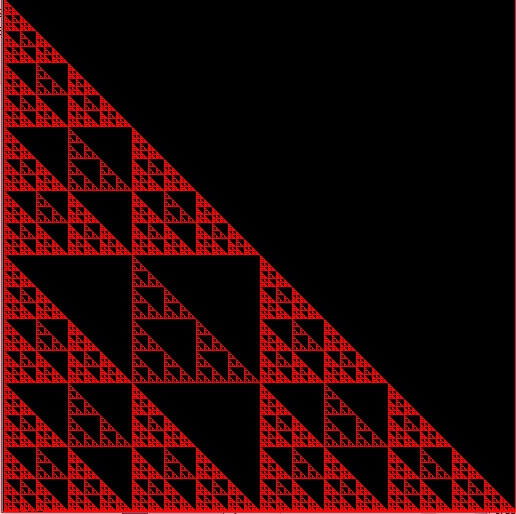
\includegraphics[scale=0.5]{Screens/noPrim.jpg}
	\captionof{figure}{Ausgabe mit Modulo 4}
	\label{fig:noprim}
\end{center}
Es fällt beim Vergleich der Ausgaben zunächst auf, dass bei Primzahlen am unteren Rand nur Teile von Dreiecken vorhanden sind (Siehe gelbe Pfeile in Abbildung 3.1). Wohingegen bei Zahlen die keine Primzahl sind, alle entstandenen Dreiecke vollständig im Bild sind. Eine weitere Besonderheit bei der Ausgabe mit Primzahlen ist: Über den Dreiecken sind so viele kleine Dreiecke in Reihe wie die um eins verringerte Zahl mit der Modulo gerechnet wurde. Das grünes Rechteck in Abbildung 3.1. Zuletzt ist anzumerken, dass die Ausgabe bei Primzahlen geordneter wirkt, wohingegen sie bei allen anderen Zahlenwerte deutlich fragmentierter wirkt.
\subsection*{c)}
Werden wir machen!

\end{document}